\documentclass{standalone}
\usepackage{tikz}
\begin{document}
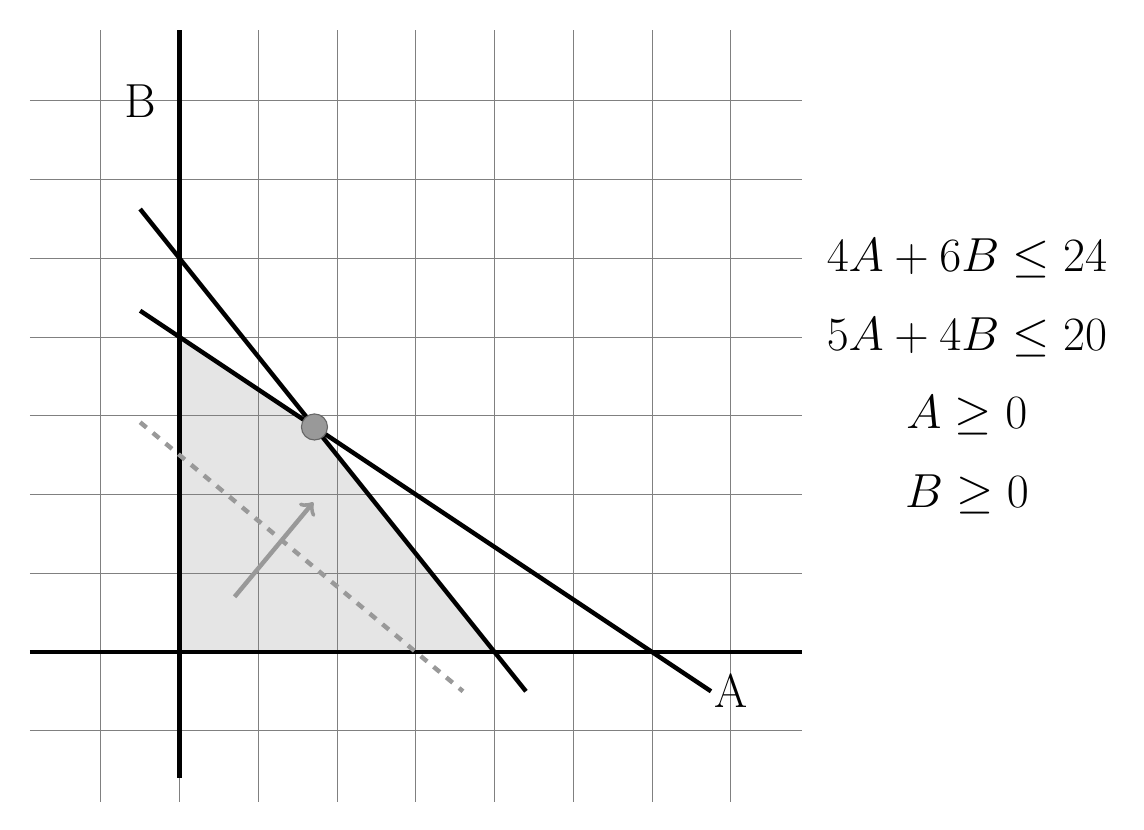
\begin{tikzpicture}
\draw[draw=none, fill=black!10] (0, 0) -- (0, 4) -- (12/7, 20/7) -- (4, 0) -- cycle;
\draw[step=1cm,gray,very thin] (-1.9,-1.9) grid (7.9,7.9);
\draw[ultra thick] (-1.9, 0) -- (7.9, 0);
\draw[ultra thick] (0, -1.6) -- (0, 7.9);
\node at (7, -0.5) {\LARGE A};
\node at (-0.5, 7) {\LARGE B};
\draw[ultra thick, black] (-0.5, 13/3) -- (27/4, -0.5);
\draw[ultra thick, black] (-0.5, 45/8) -- (22/5, -0.5);
\node[text=black] at (10, 5) {\LARGE $4A + 6B \leq 24$};
\node[text=black] at (10, 4) {\LARGE $5A + 4B \leq 20$};
\node[text=black] at (10, 3) {\LARGE $A \geq 0$};
\node[text=black] at (10, 2) {\LARGE $B \geq 0$};

\draw[ultra thick, black!40, dashed] (-0.5, 35/12) -- (18/5, -0.5);
\draw[ultra thick, ->, black!40] (0.7, 0.7) -- (1.7, 1.9);
\node[style={minimum size=0.2cm,draw=black!60,fill=black!40,shape=circle}] at (12/7, 20/7) {};
\end{tikzpicture}
\end{document}
